\section{System Overview}
Figure~\ref{fig:overview}

This paper describe our system for bimanual sewing with a curved needle. We use two robots to manipulate the needle, i.e. piercing and pass from one robot to another. Two KUKA robots are mounted with needle drivers to grip the needle. In addition to these, a third robot is used to control the fabric tube. An special mandrel is designed to support the fabric tube and bound it tightly with the stent. Holes on the mandrel allow the needle to go through and hence stitch the stent and the fabric together. Our sewing task requires high accuracy and robustness. Each stitch is required to be at the exact place and have the same length. We use a vision system to guide the robot movements in order to maintain the accuracy. The needle position is tracked during the whole task. The robot movements are computed online to deliver the needle to stitch at the correct spot. The robot movements are programmed by human demonstrations.

We adopt an bimanual sewing approach: the curved needle is first carried by one robot (A) to pierce the fabric, and picked up by another robot (B) from the other side. The needle is then pulled out by the robot B and passed back to the robot A. The third robot moves to the next stitch position. These movements complete one cycle and repeat the cycle until the whole stent is sewed.

\subsection{Vision System}
As mentioned above, the needle is manipulate between two robots. During the sewing task, defect can easily occur by the slip between the needle and the needle drivers. This usually happen during the passing stage: when one robot pass the needle to another, small displacement of the optimal relative pose between the needle and the needle driver can occur. We use a stereo vision system to monitor the process and measure the displacements. Adaptive robot movements are then generated to compromise these small displacements and deliver the needle to the correct spot.

Needle tracking / re-detection

\subsection{Learning from human demonstration}

We programme the robot in a learning manner. 

\begin{enumerate}
\item{1}: Human demonstrate how to sew stent graft


\item{2}: Tracking needle (object centric approach)
\item{3}: Motion segmentation
\item{4}: Primitive motion learning
\end{enumerate}

\subsection{Task execution}

\begin{enumerate}
\item{1}: Needle pose re-detection
\item{2}: Trajectory adaptation
\end{enumerate}

\begin{figure}
\centering
{
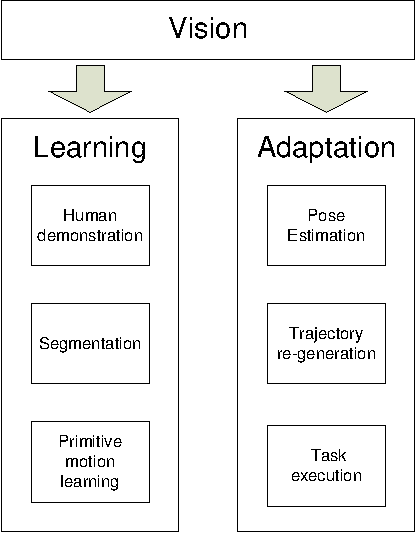
\includegraphics[width=5cm]{./fig/overview.pdf}
\caption{\scriptsize{System overview of bimanual sewing robot}}

\label{fig:overview}
}
\end{figure} 